\chapter{Основные понятия и определения теории каскадов}

Наряду с развитием технологий разделения изотопов развивается также и теория каскадов для разделения изотопных смесей. За последние десятилетия в ней достигнуты значительные успехи в части описания процессов молекулярно-селективного массопереноса при разделения многокомпонентных смесей. Предложенные модели могут быть использованы, в том числе, для изучения физических закономерностей процесса обогащения регенерированного урана, который, в отличие от природного урана, нельзя упрощенно рассматривать в качестве бинарной смеси.
Ниже, для более понятного изложения остальных частей диссертации кратко приведены основные понятия из теории каскадов для разделения многокомпонентных смесей, а также использованные в рамках диссертационного исследования модели каскадов для разделения многокомпонентных смесей.

\section{Основы теории разделения в каскадах}

% На сегодняшний день разработан обширный набор расчетных моделей, которые могут быть применены в том числе и к задаче обогащения регенерированного урана \cite{smirnovMolekulyarnoselektivnyyMassoperenosKomponentov2013}. Введем основные теоретические понятия и рассмотрим модельные каскады, релевантные задаче диссертационной работы.

\subsection{Понятие разделительной ступени}

Рассмотрим общие характеристики разделительных ступеней, предназначенных для разделения многокомпонентных изотопных смесей в газовой фазе. В качестве разделяемой изотопной смеси рассмотрена смесь, содержащая \textit{m} химически не реагирующих между собой компонентов, содержание можно определять либо мольно-долевыми концентрациями, либо массовыми $C_{i}$ ($i=1,\, 2,...,m$) \cite{sulaberidzeTeoriyaKaskadovDlya2011}. Компоненты пронумерованы в порядке возрастания массовых чисел. В рамках диссертационного исследования будут использованы массовые концентрации. При этом следует уточнить, что в случае разделения смесей изотопов тяжелых химических элементов, включая уран, численные значения массовых и мольных долей приблизительно совпадают \cite{sulaberidzeTeoriyaKaskadovDlya2011}.  Для концентраций компонентов разделяемой смеси справедливо очевидное тождество:

\begin{equation} \label{GrindEQ__1_1_} 
  \sum _{j=1}^{m}C_{j}  =1 
\end{equation} 
  
Наряду с абсолютными концентрациями $C_{i} $ часто используют относительные концентрации, определяемые по отношению к концентрации так называемого «опорного» компонента с фиксированным номером, например, \textit{k}, то есть

\begin{equation} \label{GrindEQ__1_2_} 
  R_{ik} =\frac{C_{i} }{C_{k} } , i=1,\, 2,...,m.             
\end{equation} 
  
В качестве <<опорного>> может быть выбран любой из компонентов смеси. 
Простая трехпоточная разделительная ступень имеет один входной поток и два выходных (рис. \ref{1_1}). На вход ступени поступает поток питания (производительность ступени) $L$  (в системе СИ в кг/с) с концентрациями $C_{i}$ ($i=1,\, 2,...,m$). Из ступени выходят два потока: легкая фракция (поток, обогащенный легкими компонентами) или отбор ступени $L'$ и тяжелая фракция (поток, обедненный легкими компонентами) или отвал ступени $L''$. Концентрации компонентов в этих потоках  $C'_{i} $ и $C''_{i} $, соответственно.

\begin{figure}[ht]
  \centerfloat{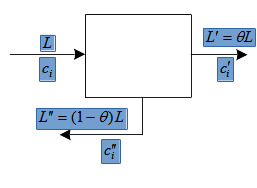
\includegraphics[scale=0.7]{images/theory/lu15087t0po}}
  \caption{Схема трехпоточной разделительной ступени }\label{1_1}
\end{figure}

Коэффициент деления потоков смеси (срез) $\theta$, парциальные потоки компонентов $G_{i} ,\; G'_{i} ,\; G''_{i}$ и срезы парциальных потоков $\phi _{i}$ можно определить по формулам:

\begin{equation} \label{GrindEQ__1_3_} 
  \theta =\frac{L'}{L} ,\; G_{i} =LC_{i} ,\; G'_{i} =L'C'_{i} ,\; G''_{i} =L''C''_{i} , 
  \end{equation} 
  \begin{equation} \label{GrindEQ__1_4_} 
  \phi _{i} =\frac{G'_{i} }{G_{i} } ,\; 1-\phi _{i} =\frac{G"_{i} }{G_{i} } ,\; i=1,2,...,m. 
  \end{equation} 

В стационарном режиме работы и в отсутствие потерь рабочего вещества потоки ступени связаны уравнениями баланса:

\begin{equation} \label{GrindEQ__1_5_} 
  L=L'+L'', 
  \end{equation} 
  \begin{equation} \label{GrindEQ__1_6_} 
  G_{i} =G'_{i} +G''_{i} , i=1,\, 2,...,m.             
\end{equation} 
  

Введенное в \ref{GrindEQ__1_3_} определение среза потоков ступени дает возможность представить уравнения \ref{GrindEQ__1_6_} в следующем виде:

\begin{equation} \label{GrindEQ__1_7_} 
  C_{i} =\theta C'_{i} +(1-\theta )C''_{i} . 
\end{equation} 

Для каждого компонента $i$ с относительной концентрацией вводят относительные коэффициенты разделения: полный $q_{ik}$, в отборе (потоке лёгкой фракции) $\alpha _{ik} $ и в отвале (потоке тяжёлой фракции) $\beta _{ik} $ и соответствующие коэффициенты обогащения $\varepsilon _{ik} ,\varepsilon '_{ik} ,\; \varepsilon ''_{ik} \; $
\[q_{ik} =\frac{R'_{ik} }{R''_{ik} } ,\; \; \alpha _{ik} =\frac{R'_{ik} }{R_{ik} } ,\; \; \beta _{ik} =\frac{R_{ik} }{R''_{ik} } ,\] 

\begin{equation} \label{GrindEQ__1_11_} 
  \begin{array}{l}
    \qquad q_{i k}=\frac{R_{i k}^{\prime}}{R_{i k}^{\prime \prime}}, \alpha_{i k}=\frac{R_{i k}^{\prime}}{R_{i k}}, \beta_{i k}=\frac{R_{i k}}{R_{i k}^{\prime \prime}} \\
    \varepsilon_{i k}=q_{i k}-1, \varepsilon_{i k}^{\prime}=\alpha_{i k}-1, \varepsilon_{i k}^{\prime \prime}=1-\frac{1}{\beta_{i k}}
    \end{array}
\end{equation} 

При разделении изотопов молекулярно-кинетическими методами, включая метод газовой центрифуги, величины относительных коэффициентов разделения можно аппроксимировать соотношениями $q_{ij} =q_{0} {}^{M_{j} -M_{i} }$, где \textit{q}${}_{0}$ – коэффициент разделения, приходящийся на единицу разности массовых чисел; \textit{M${}_{i}$, M${}_{j}$} – массовые числа $i$-го и $j$-го компонентов, соответственно \cite{sulaberidzeTeoriyaKaskadovDlya2011}.

Если $k\ne m$, то при всех $i<k$ значения всех коэффициентов разделения $q_{ik} $, $\alpha _{ik} $, $\beta _{ik} $, будут больше единицы, а при всех $i>k$ -- меньше единицы.

Полные коэффициенты разделения $q_{ik} $, как правило, не зависят от состава смеси. В некоторых случаях, что характерно для газовой центрифуги, коэффициенты $q_{ik} $ могут зависеть от коэффициента деления потоков смеси (срез) $\theta $ и от потока питания одиночного разделительного элемента (ступени) $ L $ (\ref{GrindEQ__q_}) \cite{mustafinObjectiveFunctionOptimization2019}:

\begin{equation} \label{GrindEQ__q_} 
  q_{ij} = f(\theta, L}),              
\end{equation}

В практических расчетах при определении оптимальных параметров разделительного каскада необходимо учитывать данную зависимость, конкретный вид которой может быть получен теоретически путем решения задачи конвективной диффузии для одиночного разделительного аппарата. После чего зависимость может быть уточнена на основе экспериментальных данных. 
Анализ зависимостей вида (\ref{GrindEQ__q_}) для различных газовых центрифуг показывает, что часть данной функции, определяемая величиной $\theta $ представляет собой гладкую функцию с одним экстремумом (максимумом). В теоретических исследованиях часто используют упрощенные подходы, в которых либо пренебрегают зависимостью коэффициентов разделения от какого-либо из указанных выше параметров, либо от всех, считая коэффициенты разделения одинаковыми на всех ступенях. Например, можно пренебречь зависимостью величины коэффициента разделения от $\theta $, осуществив, например, предварительное усреднение функции (\ref{GrindEQ__q_}) по этому параметру и выбрав оптимальную с точки зрения разделительной способности элемента величину потока питания $ L $. Такой подход как в случае разделения бинарных, так и многокомпонентных смесей приводит к теории так называемых «модельных каскадов» (каскадов с одинаковыми по ступеням коэффициентами разделения \cite{sulaberidzeClassificationModelCascades2020}.

Такой подход был использован и в настоящем исследовании, поэтому далее будут рассмотрены только случаи каскадов, состоящих из разделительных элементов, имеющих одинаковые коэффициенты разделения и работающих в идентичных режимах.  

В дополнение к введеным выше параметрам также используют величины $ g_{i} $, которые можно рассматривать как отношение парциальных потоков компонентов в лёгкой и тяжёлой фракциях, покидающих ступень:

\begin{equation} \label{GrindEQ__1_13_} 
  g_{i} =\frac{\phi _{i} }{1-\phi _{i} } =\frac{G'_{i} }{G''_{i} } , i\ne k, 
  \end{equation} 
  \begin{equation} \label{GrindEQ__1_14_} 
  g_{k} =\frac{\phi _{k} }{1-\phi _{k} } =\frac{G'_{k} }{G''_{k} } .           
\end{equation} 

Нетрудно показать, что :

\begin{equation} \label{GrindEQ__1_18_} 
  L=\sum _{j=1}^{m}L_{i}  =\sum _{j=1}^{m}\frac{g_{i} +1}{g_{i} }  L_{i} ',               
  \end{equation} 
  \begin{equation} \label{GrindEQ__1_19_} 
  C_{i} =\frac{g_{i} +1}{g_{i} } \frac{L_{i} '}{L} ,         
  \end{equation} 
  

\subsection{Симметричный противоточный каскад и система уравнений, описывающих для него массоперенос в общем виде}

Как известно, при практической реализации многих методов разделения используют многоступенчатые разделительные установки, называемые каскадами \cite{sulaberidzeTeoriyaKaskadovDlya2011}. Подобные установки представляют собой последовательно соединенные ступени, состоящие из параллельно соединенных разделительных элементов, в частности газовых центрифуг. 
Cуществуют различные способы коммутации ступеней в разделительных каскадах. Одним из наиболее часто используемым и рассматриваемом в теоретических исследованиях является так называемый способ симметричного соединения ступеней в противоточной схеме (рис. \ref{1_2}). Рассмотрим схему такого каскада, имеющего один входящий поток питания $F$ и два выходящих: отбор $P$, обогащенный самым легким компонентом и отвал W, обогащенный самым тяжелым компонентом. Потоки $F$, $P$, $W$ и концентрации компонентов в них $C_{i}^{F} ,\; \; C_{i}^{P} ,\; \; C_{i}^{W} \; \; (i=1,\; 2,...,m)$ являются внешними параметрами каскада. Следует заметить, что в случае разделения многокомпонентных смесей понятия «отбор» и «отвал» условны, поскольку ценный компонент может обогащаться как вместе с самым легким компонентом смеси, так и вместе с самым тяжелым.

\begin{figure}[ht]
  \centerfloat{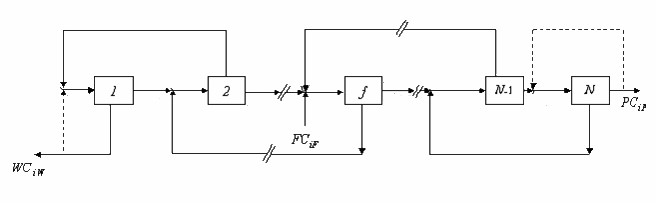
\includegraphics[scale=0.7]{images/theory/2}}
  \caption{Схема соединения ступеней в симметрично-противоточном каскаде}\label{1_2}
\end{figure}

В стационарном режиме работы и в отсутствии потерь рабочего вещества на ступенях каскада, внешние параметры каскада должны удовлетворять уравнениям материального баланса

\begin{equation} \label{GrindEQ__1_21_} 
  \begin{array}{l} {\quad \quad \quad \quad F=P+W,} \\ {FC_{i}^{F} =PC_{i}^{P} +WC_{i}^{W} ,\; i=1,2,...,m.} \end{array} 
\end{equation} 

Ступени каскада пронумерованы последовательно от $s=1$ на отвальной ступени каскада до $s=N$ на отборной ступени. Считаем, что внешнее питание каскада (\textit{F}) подают на вход ступени с номером $f$. Внутренние параметры произвольной ступени с номером \textit{s} ($L_{s} $, $L'_{s} ,$ $L''_{s} ,$ $G_{i,s} ,$ $G'_{i,s} ,$ $G''_{i,s} $), где $L$ -- потоки вещества, а $G$ -- парциальные потоки (изотопов с индексами $i$) в стационарном режиме работы каскада, в отсутствие потерь рабочего вещества на ступенях каскада связаны уравнениями \ref{GrindEQ__1_5_},  \ref{GrindEQ__1_6_}.

Уравнения баланса в «узлах» (точках соединения межступенных потоков) при симметричном соединении ступеней имеют вид:

\begin{equation} \label{GrindEQ__1_24_} 
  L_{s} =\theta _{s-1} L_{s-1} +(1-\theta _{s+1} )L_{s+1} ,\; \; s=1,\, 2,...,f-1,\, f+1,...,N, 
  \end{equation} 
  \begin{equation} \label{GrindEQ__1_25_} 
  \begin{array}{l} {L_{s} C_{i,s} =\theta _{s-1} L_{s-1} C'_{i,s-1} +(1-\theta _{s+1} )L_{s+1} C''_{i,s+1} ,\; \; s=1,\, 2,...,f-1,\, f+1,...,N,} \\ {\; \; \; \; \; \; \; \; \; \; \; \; \; \; \; \; \; \; \; \; \; \; \; \; \; \; \; \; \; \; \; \; \; \quad \quad \quad \quad \quad \; \; \; \; \; \; \; \; \; \; \; \; \; \quad \quad \quad \; \; \; \; \; \; \; \; \; \; \; \; \; \quad \quad \quad \; \; \; \; \; \; \; \; \; \; \; \; \; \quad \quad \; \quad i=1,\, 2,...,m.} \end{array} 
  \end{equation} 

Для ступени подачи питания $f$ аналогичные уравнения выглядят так:

\begin{equation} \label{GrindEQ__1_26_} 
  L_{f} =\theta _{f-1} L_{f-1} +(1-\theta _{f+1} )L_{f+1} +F, 
  \end{equation} 
  \begin{equation} \label{GrindEQ__1_27_} 
  L_{f} C_{i,f} =\theta _{f-1} L_{f-1} C'_{i,f-1} +(1-\theta _{f+1} )L_{f+1} C''_{i,f+1} +FC_{i}^{F} ,\quad i=\overline{1,m}.            
\end{equation}

Внешние и внутренние параметры каскада связаны граничными условиями

\begin{equation} \label{GrindEQ__1_28_} 
  L_{0} =L'_{0} =L''_{0} =L_{N+1} =L'_{N+1} =L''_{N+1} =0, 
  \end{equation} 
  \begin{equation} \label{GrindEQ__1_29_} 
  L'_{N} =\theta _{N} L_{N} =P,        
  \end{equation} 
  \begin{equation} \label{GrindEQ__1_30_} 
  L''_{1} =(1-\theta _{1} )L_{1} =W,        
  \end{equation} 
  \begin{equation} \label{GrindEQ__1_31_} 
  C'_{N} =C_{i}^{P} ,\; i=1,\; \; 2,...,m, 
  \end{equation} 
  \begin{equation} \label{GrindEQ__1_32_} 
  C''_{1} =C_{i}^{W} ,\; i=1,\; \; 2,...,m, 
  \end{equation} 
  \begin{equation} \label{GrindEQ__1_33_} 
  G'_{i,N} =PC_{i}^{P} ,\; i=1,\; \; 2,...,m, 
  \end{equation} 
  \begin{equation} \label{GrindEQ__1_34_} 
  G''_{i,1} =WC_{i}^{W} ,\; i=1,\; \; 2,...,m. 
\end{equation} 

Соотношения (\ref{GrindEQ__1_21_})--(\ref{GrindEQ__1_34_}) описывают простейшую физико-математическую модель противоточного симметричного каскада, предназначенного для разделения многокомпонентной смеси. Анализ данной системы показывает, что она представляют собой системы нелинейных разностных уравнений относительно функций $C_{i,s}$. Существенной проблемой при решении подобных систем является то, что в эти уравнения (либо в их граничные условия) входят значения концентраций, которые неизвестны заранее и должны быть определены из решения этих же уравнений. В общем случае, системы (\ref{GrindEQ__1_24_})--(\ref{GrindEQ__1_27_}), (\ref{GrindEQ__1_35_})--(\ref{GrindEQ__1_38_}) или (\ref{GrindEQ__1_39_})--(\ref{GrindEQ__1_40_}) требуют использования численных методов.

Трудности решения (\ref{GrindEQ__1_24_})--(\ref{GrindEQ__1_34_}) в общем случае, стимулировали развитие упрощенных подходов, которые позволяют получить аналитическое решение для данных систем при введении определенных предположений. Полученные в результате таких упрощений физико-математические модели симметрично-противоточного каскада сохраняют закономерности молекулярно-селективного массопереноса, но позволяют заметно упростить соответствующие расчетные процедуры для определения оптимальных параметров каскада. Такие каскады получили название модельных \cite{minenkoTeoriiKaskadovDlya1965, delagarzaMulticomponentIsotopeSeparation1961, zhigalovskiyLekcionnyeMaterialyPo1999, kolokoltsovDesignCascadesSeparating1970, kolokolcovVoprosuPostroeniiKaskadov1970, minenkoPredelnoeObogashcheniePromezhutochnyh1972, yamamotoMulticomponentIsotopeSeparating1978, wuStudyMulticomponentIsotope, borisevichRascheteKaskadovDopolnitelnym1993, woodCriterionEffiencyMultiisotope1999, sulaberidzeOsobennostiObogashcheniyaKomponentov2006, sazykinKvaziidealnyeKaskadyDlya2000, sulaberidzeSravnenieOptimalnyhModelnyh2008}.

Как показали результаты теоретического анализа модельные каскады фактически представляют собой частный случай рассмотренного выше симметрично-противоточного каскада, отвечающий условию постоянства по его длине относительных коэффициентов разделения \cite{sulaberidzeClassificationModelCascades2020}. Такое предположение в ряде случаев позволяет получить аналитическое решение общих уравнений симметрично-противоточного каскада, тем самым упростив изучения физических закономерностей массопереноса в каскадах для разделения многокомпонентных смесей. 
Ниже кратко рассмотрены предложенные на текущий момент модельные каскады.

\subsection{«Квазиидеальный» каскад}

Рассмотрим случай симметричного противоточного каскада с постоянными по его длине относительными коэффициентами разделения $q_{ik} ,\; \alpha _{ik} ,\; \beta _{ik} $ $(i=1,\; 2,...,m;$ \textit{k}--номер «опорного» компонента). Условие постоянства относительных коэффициентов разделения обеспечивает выполнение условия постоянства величин \textit{g${}_{i}$} и $\phi _{i} $. Следовательно, соотношения (\ref{GrindEQ__1_24_})--(\ref{GrindEQ__1_27_}) приводятся к виду \cite{sulaberidzeTeoriyaKaskadovDlya2011}:

\begin{equation} \label{GrindEQ__1_52_} 
  G'_{i} (s-1)+\frac{1}{g_{i} } G'_{i} (s+1)-\frac{g_{i} +1}{g_{i} } G'_{i} (s)+\delta _{sf} Fc_{iF} =0,\; \; i\ne k, 
  \end{equation} 
  \begin{equation} \label{GrindEQ__1_53_} 
  G'_{k} (s-1)+\frac{1}{g_{k} } G'_{k} (s+1)-\frac{g_{k} +1}{g_{k} } G'_{k} (s)+\delta _{sf} Fc_{kF} =0, 
  \end{equation}

где $s$ – текущий номер ступени, отсчитываемый от «тяжелого» конца каскада к его «легкому» концу $\delta _{sf} =\left\{\begin{array}{l} {0,\; \; s\ne f} \\ {1,\; \; s=f} \end{array}\right. $

Уравнения (\ref{GrindEQ__1_52_})--(\ref{GrindEQ__1_53_}) представляют собой линейные разностные уравнения второго порядка относительно неизвестных функций $G'_{i} (s)$. Граничные условия для них имеют вид:

\begin{equation} \label{GrindEQ__1_54_} 
  \left\{\begin{array}{l} {G'_{i} (0)=G'_{i} (N+1)=0,\; \; i=1,\; 2,...,m} \\ {G'_{i} (N)=PC_{i}^{P} ,\; \; i=1,\; 2,...,m} \\ {G'_{i} (1)=g_{i} WC_{i}^{W} ,\; \; i\ne k} \\ {G''_{k} (1)=g_{k} WC_{i}^{W} .} \end{array}\right.  
\end{equation} 

Ступени с номерами $s=1$ и $s=N$ являются крайними ступенями каскада, что делает возможным формально записать $G'_{i} (0)=G'_{i} (N+1)=0$.

Решив (\ref{GrindEQ__1_52_}) и (\ref{GrindEQ__1_53_}), а также используя уравнения баланса (\ref{GrindEQ__1_21_}) и граничные условия (\ref{GrindEQ__1_54_}), можно получить уравнения связи внешних параметров такого каскада с длинами его секций и параметрами ступени. В итоге:

\begin{equation} \label{GrindEQ__1_55_} 
  \frac{P}{F} =\sum _{j=1}^{m}C_{j}^{F} \frac{1-g_{j}^{-f} }{1-g_{j}^{-N-1}} ,\; \; s=f,...,N ,                                                  
  \end{equation} 
  \begin{equation} \label{GrindEQ__1_56_} 
  \frac{W}{F} =\sum _{j=1}^{m}C_{j}^{F} \frac{g_{j}^{N+1-f} -1}{g_{j}^{N+1} -1} ,\; \; s=1,...,f-1 ,                                            
\end{equation}

\begin{equation} \label{GrindEQ__1_57_} 
  C_{i}^{P}=C_{i}^{F} \frac{1-g_{i}^{-f}}{1-g_{i}^{-N-1}} / \sum_{j=1}^{m} C_{j}^{F} \frac{1-g_{j}^{-f}}{1-g_{j}^{-N-1}}, i=1,2, \ldots, m                             
\end{equation}

\begin{equation} \label{GrindEQ__1_58_} 
  C_{i}^{W}=C_{i}^{F} \frac{g_{i}^{N+1-f}-1}{g_{i}^{N+1}-1} / \sum_{j=1}^{m} C_{j}^{F} \frac{g_{j}^{N+1-f}-1}{g_{j}^{N+1}-1}, i=1,2, \ldots, m                         
\end{equation} 

Далее, распределение потока $L(s)$, концентраций компонентов и коэффициента деления потоков по ступеням каскада можно определить по формулам \cite{sulaberidzeTeoriyaKaskadovDlya2011}:

\begin{equation} \label{GrindEQ__1_59_} 
L(s)=\sum_{j=1}^{m} G_{j}^{\prime}(s) \frac{1+g_{j}}{g_{j}}=\left\{\begin{array}{c}
  P \sum_{j=1}^{m} \frac{g_{j}+1}{g_{j}-1} C_{j}^{P}\left(1-g_{j}^{s-N-1}\right), s=f, \ldots, N \\
  W \sum_{j=1}^{m} \frac{g_{j}+1}{g_{j}-1} C_{j}^{\pi}\left(g_{j}^{s}-1\right), s=1, \ldots, f-1
  \end{array}\right.
\end{equation} 

\begin{equation} \label{GrindEQ__1_60_} 
C_{i} (s)=\frac{1+g_{j} }{g_{j} } \cdot \frac{G''_{i} (s)}{G_{i} (s)} =\left\{\begin{array}{l} {\frac{C_{i}^{P} \frac{g_{j} }{g_{j} -1} \left(1-g_{j}^{s-N-1} \right)}{\sum _{j=1}^{m}\frac{g_{j} +1}{g_{j} -1}  C_{j}^{P} \left(1-g_{j}^{s-N-1} \right)} ,\; \; s=f,...,N,} \\ {\; \frac{C_{i}^{W} \frac{g_{j} }{g_{j} -1} \left(g_{j}^{s} -1\right)}{\sum _{j=1}^{m}\frac{g_{j} +1}{g_{j} -1}  C_{j}^{W} \left(g_{j}^{s} -1\right)} ,\; \; s=1,...,f-1,} \end{array}\right.  
\end{equation} 

\begin{equation} \label{GrindEQ__1_61_} 
\begin{array}{l} {\theta (s)=\frac{\sum _{j=1}^{m}G'_{j} (s) }{\sum _{j=1}^{m}G_{j} (s) } =\left\{\begin{array}{l} {\frac{\sum _{j=1}^{m}\frac{g_{j} }{g_{j} -1} C_{j}^{P} \left(1-g_{j}^{s-N-1} \right) }{\sum _{j=1}^{m}\frac{g_{j} +1}{g_{j} -1}  C_{j}^{P} \left(1-g_{j}^{s-N-1} \right)} ,\; \; s=f,...,N,} \\ {\; \frac{\sum _{j=1}^{m}\frac{g_{j} }{g_{j} -1} C_{j}^{W} \left(g_{j}^{s} -1\right) }{\sum _{j=1}^{m}\frac{g_{j} +1}{g_{j} -1}  C_{j}^{W} \left(g_{j}^{s} -1\right)} ,\; \; s=1,...,f-1.} \end{array}\right. } \\ {\; } \end{array} 
\end{equation}

Формулу для расчета относительного суммарного потока в каскаде легко получить, суммируя (\ref{GrindEQ__1_59_}) по всем ступеням каскада

\begin{equation} \label{GrindEQ__1_62_} 
  \sum _{s=1}^{N}\frac{L(s)}{P} =\sum _{i=1}^{m}\left\{\frac{g_{i} +1}{g_{i} -1} \left[\frac{W}{P} C_{i}^{W} (f)+C_{i}^{P} \left(N+1-f\right)\right]\right\}  .   
\end{equation} 
  
Рассмотренный выше каскад отличается тем, что относительные коэффициенты разделения $q_{ik} ,\; \alpha _{ik} ,\; \beta _{ik} $ (и, соответственно, срезы парциальных компонентов $\phi _{i} ,\; \; \phi _{k} $ и параметры $g_{i} $, $g_{k} $) остаются постоянными по длине каскада. Для таких каскадов в работе \cite{sazykinKvaziidealnyeKaskadyDlya2000} был введен термин «квазиидеальный» каскад.

\subsection{Каскад с несмешиванием относительных концентраций двух заданных компонентов смеси (R-каскад)}

Рассмотрим каскад, в котором выполняется несмешивание относительных концентраций $n$-го и $k$-го компонентов смеси. Данная каскадная модель является аналогом используемого в теории разделения бинарных смесей «идеального» каскада, в «узлы» которого входят потоки с одинаковой концентрацией компонентов. Условие несмешения по относительным концентрациям $n$-го и $k$-го компонентов можно записать в виде:

\begin{equation} \label{GrindEQ__1_68_} 
  R'_{nk} (s-1)=R_{nk} (s)=R''_{nk} (s+1).                                                 
\end{equation} 

Подобная модель получила в теории название - R-каскад \cite{sulaberidzeTeoriyaKaskadovDlya2011}. Отметим, что R-каскады могут быть построены как в случае «слабого обогащения», так и для немалых обогащений на ступени. Рассмотрим второй из указанных случаев, как соответствующий разделению изотопов в газовых центрифугах.
Вследствие (\ref{GrindEQ__1_68_}) легко показать, что коэффициенты $\alpha _{nk} $ и $\beta _{nk} $ совпадают для двух соседних ступеней. При постоянных полных коэффициентах разделения равенство:

\begin{equation} \label{GrindEQ__1_69_} 
  \alpha _{nk} =\beta _{nk} =\sqrt{q_{nk} }  
\end{equation} 

приводит к каскаду со ступенями симметричными относительно пары компонентов с номерами $n$ и $k$. При этом на всех ступенях каскада $\alpha _{ik} \ne \beta _{ik} \; (i\ne n)$. Учитывая, сказанное выше, (\ref{GrindEQ__1_55_})--(\ref{GrindEQ__1_58_}) могут быть переписаны виде:
  

\begin{equation} \label{GrindEQ__1_70_} 
  \frac{P}{F} =\sum _{j=1}^{m}C_{j}^{F} \frac{(R_{nk}^{W} )^{-d_{j} } -(R_{nk}^{F} )^{-d_{j} } }{(R_{nk}^{W} )^{-d_{j} } -(R_{nk}^{P} )^{-d_{j} } }  ,                                            
  \end{equation} 
  \begin{equation} \label{GrindEQ__1_71_} 
  \frac{W}{F} =\sum _{j=1}^{m}C_{j}^{F} \frac{(R_{nk}^{F} )^{-d_{j} } -(R_{nk}^{P} )^{-d_{j} } }{(R_{nk}^{W} )^{-d_{j} } -(R_{nk}^{P} )^{-d_{j} } }  ,                                        
\end{equation} 

\begin{equation} \label{GrindEQ__1_72_} 
  C_{i}^{P}=C_{i}^{F} \frac{\left(R_{n k}^{W}\right)^{-d_{i}}-\left(R_{n k}^{F}\right)^{-d_{i}}}{\left(R_{n k}^{W}\right)^{-d_{i}}-\left(R_{n k}^{P}\right)^{-d_{i}}} / \sum_{j=1}^{m} C_{j}^{F} \frac{\left(R_{n k}^{W}\right)^{-d_{j}}-\left(R_{n k}^{F}\right)^{-d_{j}}}{\left(R_{n k}^{W}\right)^{-d_{j}}-\left(R_{n k}^{P}\right)^{-d_{j}}}
\end{equation} 

\begin{equation} \label{GrindEQ__1_73_} 
  C_{i}^{W}=C_{i}^{F} \frac{\left(R_{n k}^{F}\right)^{-d_{i}}-\left(R_{n k}^{P}\right)^{-d_{i}}}{\left(R_{n k}^{W}\right)^{-d_{i}}-\left(R_{n k}^{P}\right)^{-d_{i}}} / \sum_{j=1}^{m} C_{j}^{F} \frac{\left(R_{n k}^{F}\right)^{-d_{j}}-\left(R_{n k}^{P}\right)^{-d_{j}}}{\left(R_{n k}^{W}\right)^{-d_{j}}-\left(R_{n k}^{P}\right)^{-d_{j}}}
\end{equation} 

\begin{equation} \label{GrindEQ__1_74_} 
  d_{i} =\frac{\ln q_{ik} }{\ln g_{n} } -1,              
\end{equation}

, где $R_{n k}^{F}$, $R_{n k}^{W}$ и $R_{n k}^{P}$ -- относительные концентрации целевого компонента в потоках $F$, $W$, и $P$, соответственно.

Для молекулярно-кинетических методов разделения соотношения (\ref{GrindEQ__1_15_})--(\ref{GrindEQ__1_16_}) можно записать в следующем виде:

\begin{equation} \label{GrindEQ__1_75_} 
  g_{k} =q_{0}^{-\frac{M_{k} -M_{n} }{2} } ,        
  \end{equation} 
  \begin{equation} \label{GrindEQ__1_76_} 
  g_{i} =q_{0}^{M^{*} -M_{i} } ,        
\end{equation} 

, где $M^{*} =\frac{M_{n} +M_{k} }{2} $.

Из (\ref{GrindEQ__1_75_})--(\ref{GrindEQ__1_76_}) непосредственно следует, что для всех компонентов с $M_{i} $$\mathrm{<}$$M^{*} $ величины $g_{i} $$\mathrm{>}$1, если же $M_{i} $$\mathrm{>}$$M^{*} $, то $g_{i} $$\mathrm{<}$1. Из соотношений (\ref{GrindEQ__1_72_}) и (\ref{GrindEQ__1_73_}) при выполнении условий $N-f+1>>1,\; \; f-1>>1$ («длинный каскад») следует, что в таком R-каскаде компоненты с $g_{i} $$\mathrm{>}$1 ($M_{i} $$\mathrm{<}$$M^{*} $ обогащаются к «легкому» выходящему потоку каскада, а компоненты с $g_{i} $$\mathrm{<}$1 ($M_{i} $$\mathrm{>}$$M^{*}$ обогащаются к «тяжелому» выходящему потоку каскада. Следовательно, величина параметра $M^{*}$ полностью определяет направление обогащения компонентов смеси в R-каскаде. 

Суммарный поток R-каскада равен \cite{sulaberidzeTeoriyaKaskadovDlya2011}:

\begin{equation} \label{GrindEQ__1_77_} 
  \sum _{s=1}^{N}L(s) =\sum _{j=1}^{m}\frac{PC_{j}^{P} \ln R_{nk}^{P} +WC_{j}^{W} \ln R_{nk}^{W} -FC_{j}^{F} \ln R_{nk}^{F} }{\frac{g_{j} -1}{g_{j} +1} \ln g_{n} }  .               
\end{equation} 

Отметим, что как следует из приведенных выше соотнршений, выбор опорного компонента определяет величину $M^{*}$. При этом, строго говоря, величина $M^{*}$ для любой $m$-компонентной смеси является дискретной функцией номера опорного компонента и, соответственно, имеет ограниченный набор допустимых значений, определяемых возможным количеством «опорных» компонентов смеси. В \cite{sulaberidzeSravnenieOptimalnyhModelnyh2008} предложено формально ввести в рассмотрение «виртуальные» компоненты с исчезающее малой концентрацией (на несколько порядков меньше наименьшей концентрации «реальных» компонентов смеси) и с массовыми числами, лежащими в пределах от \textit{M${}_{1}$} до \textit{M${}_{m}$}. В этом случае значение M* может принимать любые значения в интервале от \textit{M${}_{1}$} до \textit{M${}_{m}$}. Это позволяет построить кривую зависимости суммарного потока в каскаде от величины $M^{*}$ и найти ее минимум.  
\end{enumerate}
  
Тем самым, данный подход позволяет из бесконечного множества набора параметров R-каскадов, обеспечивающих получение заданных концентраций целевого компонента в выходящих потоках, выбрать параметры такого R-каскада, который отвечает минимуму величины суммарного потока \cite{sulaberidzeSravnenieOptimalnyhModelnyh2008}. При этом полученные параметры такого R-каскада будет незначительно (менее, чем на 1\%) отличаться от параметров оптимального по величине суммарного потока каскада (при заданных концентрациях целевого компонента в потоках отбора и отвала) \cite{songComparativeStudyModel2010}. Такой R-каскад можно рассматривать как наилучший или «эталонный». С физической точки зрения варьировании величины $M^{*}$ означает варьирование или «перебор» различных вариантов функций распределения потока питания ступеней каскада, которые, в свою очередь, определяют закономерности массопереноса компонентов по длине каскада.

Приведенные выше свойства каскада с несмешиванием по относительным концентрациям выбранной пары компонентов (R-каскада) делают его очень удобным для численного моделирования процессов молекулярно-селективного массопереноса в каскаде казовых центрифуг для разделения многокомпонентных смесей, таких как регенерированный уран. Поскольку основные цельи диссертационной работы связаны с поиском эффективного способа обогащения регенерированного урана в условиях его многократного рецикла, то выбор модельных каскадов в качестве инструмента исследования выглядит целесообразно. 
